\section{Evaluation}\label{sec:eval}

%  \milind{Putting this comment back :-) Need to intro evaluation here: 
%  1. what research questions we're trying to answer, and why. Each RQ (or two) is going to correspond to a subsection of the evaluation.
%  2. high level overview of what we're going to evaluate to answer those questions
%  3. what platforms we're using to do the evaluation
%  }

In this evaluation, we aim to answer the following questions:

\raghav{flipped the first two around so its in order :)}
\begin{enumerate}
    \item {\bf How effective is \system's vectorization?} To answer this, we count the number of instructions generated in the vector code compared to the scalar code. (Section~\ref{sec:compilation-stuff})
    \item {\bf How much speedup does compiling with \system get us?} To address this, we compile several realistic benchmarks and measure the speedup of the vectorized code over scalar execution. (Section~\ref{sec:speedups})
    \item {\bf How well do \system's schedules compare to hand-optimized code?} We compare the run times of various hand-optimized benchmarks to the run time of the vector code that \system generates for them. (Section~\ref{sec:expert-comparison})
    \item {\bf To what extent does the data layout chosen by the programmer affect \system's ability to vectorize?} We conduct a case study exploring various data layout schemes for a $3\times 3$ matrix multiply, and measure the vectorization speedup for each layout. (Section~\ref{sec:effects-of-data-layout})
   \item {\bf How effective is the layout/schedule co-optimization strategy?} We track the progress of the schedule-search procedure over time for various levels of data layout optimization. (Section~\ref{sec:search-and-cooptimization})
\end{enumerate}

\subsection{Computational Kernels}

%\raghav{spot-check my tenses?}
To assess \system's ability to vectorize general applications, we use a suite of benchmarks that represent a spectrum of both regular and irregular computations, as well as ones that are both sparse and dense in terms of data reuse.
While there is not currently a standard benchmark suite on which to evaluate FHE-based compilers, we choose a set of benchmarks similar\footnote{While we do not have access to Porcupine's actual benchmarks for a direct comparison, their polynomial regression corresponds to our matrix multiply, their L2 distance correpsonds to our point cloud distance, and most of their image processing kernels are specific convolutions (i.e. plaintext kernels), while we evaluate on generic convolutions. The input sizes of our benchmarks are comparable to those of Porcupine's.} to those used by Porcupine~\cite{Porcupine}, representing a spectrum of both regular and irregular computations, as well as ones that are both sparse and dense in terms of data reuse.

%\raghav{I'm hesitant to say sparse because that means something different}. \milind{Give a couple of sentence description of each, and also say whether we're classifying this as regular/irregular or dense/sparse, and why. Then you can just move the extra stuff about decision tree into the list, too}

The benchmarks are as follows:
%\raghav{I think the wording could be fixed here but I'm not sure how.}
\begin{enumerate}[label=\arabic*.]
    \item Multiplying two matrices. We do this with $2\times 2$ matrices (regular, little data reuse) and $3\times 3$ matrices (regular, some substantial data reuse). %Matrix multiply ($2\times 2$ and $3\times 3$): the $3\times 3$ matrix multiply is somewhat data-dense, since each input is used three times.
    \item Vector dot product, with vector sizes of 3, 6, and 10 (all of these are regular with no data reuse).
    \item 1D convolution. We do this with a vector of size 4 and a kernel of size 2, and with a vector of size 5 and a kernel of size 3. Both of these are regular and have little data reuse.
    \item Point cloud distances (Given a set of points, compute the square of every pairwise Euclidean distance). We do this for 3, 4, and 5 points. These are all regular but have some substantial data reuse, especially in the 5-point case.
    \item Sorting a list of size 3. This benchmark implements the sort as a ``decision tree'', taking as input three ciphertexts representing pairwise comparison results and six ciphertext ``labels'' representing possible arrangements of the sorted list. In particular, each of the three comparison results gets used in multiple branches of the tree. ``grouped'' here means the data layout groups the three comparisons into one vector and the six labels into another. This is irregular, and the grouped versions have data reuse.
    \item Finding the maximum element in a list of size 5. This benchmark takes as input five ciphertexts representing the elements of the list, and ten ciphertexts representing pairwise comparison results. Similar to the sorting benchmark, this is irregular, and the grouped versions have data reuse.
\end{enumerate}

%\raghav{redundant?}
%(Notice that the decision tree benchmark contains irregular computation, and the packed decision tree, all the point cloud distances, and the $3\times 3$ matrix multiply are relatively dense in terms of data reuse).

To investigate the effect of data replication we used three different replication strategies for each benchmark: 

\begin{enumerate}[label=(\roman*)]
\item {\em unreplicated}, where each input appears in only one input vector, and hence must be used by multiple operations in the circuit.
\item {\em partially replicated} in which one of the two inputs is fully replicated---and hence each operation that requires that input gets its own copy, obviating the need for data movement---while the other is not.
\item {\em fully replicated} in which both inputs are fully replicated. 
\end{enumerate}
Note that for dot product, replication makes no difference as each input is used exactly once.

\subsection{Costs and Effects of Vector Compilation}\label{sec:compilation-stuff}

\begin{table*}
	\small
	\centering
    \caption{Compilation time in seconds, as well as instruction counts in the scalar (SAdd, SSub, SMul) and vector (VAdd, VSub, VMul, Rot, Blend) code, and the ideal speedup (work/span). Note that ideal speedup considers rotates and blends to be free.}\label{tab:big-ass}
    \vspace{-0.5em}
    \begin{tabular}{lcccccccc}
    \toprule
    Benchmark & Time (s) & SAdd + SSub & SMul & VAdd + VSub & VMul & Rot & Blend & Ideal Speedup\\\midrule
    conv.4.2.un & 97 & 3 & 6 & 2 & 1 & 4 & 4 & 5.73\\
    conv.4.2.partially & 80 & 3 & 6 & 2 & 1 & 2 & 1 & 5.73\\
    conv.4.2.fully & 71 & 3 & 6 & 2 & 1 & 1 & 2 & 5.73\\
    \midrule
    conv.5.3.un & 206 & 6 & 9 & 3 & 1 & 7 & 5 & 8.0\\
    conv.5.3.partially & 211 & 6 & 9 & 4 & 1 & 4 & 3 & 8.0\\
    conv.5.3.fully & 208 & 6 & 9 & 4 & 1 & 2 & 3 & 8.0\\
    \midrule
    dist.3.un & 228 & 18 & 9 & 1 & 1 & 4 & 6 & 9.82\\
    dist.3.partially & 233 & 18 & 9 & 1 & 1 & 4 & 6 & 9.82\\
    dist.3.fully & 226 & 18 & 9 & 2 & 2 & 2 & 7 & 9.82\\
    \midrule
    dist.4.un & 425 & 32 & 16 & 2 & 2 & 6 & 8 & 17.45\\
    dist.4.partially & 432 & 32 & 16 & 2 & 2 & 6 & 8 & 17.45\\
    dist.4.fully & 463 & 32 & 16 & 2 & 2 & 4 & 8 & 17.45\\
    \midrule
    dist.5.un & 619 & 50 & 25 & 2 & 2 & 13 & 10 & 27.27\\
    dist.5.partially & 629 & 50 & 25 & 2 & 2 & 13 & 10 & 27.27\\
    dist.5.fully & 609 & 50 & 25 & 2 & 2 & 9 & 10 & 27.27\\
    \midrule
    dot.3.un & 10 & 2 & 3 & 3 & 1 & 2 & 0 & 2.67\\
    dot.3.partially & 10 & 2 & 3 & 3 & 1 & 2 & 0 & 2.67\\
    dot.3.fully & 10 & 2 & 3 & 3 & 1 & 2 & 0 & 2.67\\
    \midrule
    dot.6.un & 159 & 5 & 6 & 4 & 1 & 3 & 2 & 5.0\\
    dot.6.partially & 154 & 5 & 6 & 4 & 1 & 3 & 2 & 5.0\\
    dot.6.fully & 156 & 5 & 6 & 4 & 1 & 3 & 2 & 5.0\\
    \midrule
    dot.10.un & 254 & 9 & 10 & 6 & 1 & 5 & 4 & 7.79\\
    dot.10.partially & 257 & 9 & 10 & 6 & 1 & 5 & 4 & 7.79\\
    dot.10.fully & 251 & 9 & 10 & 6 & 1 & 5 & 4 & 7.79\\
    \midrule
    mm.2.un & 176 & 4 & 8 & 2 & 1 & 3 & 2 & 7.64\\
    mm.2.partially & 171 & 4 & 8 & 2 & 1 & 2 & 1 & 7.64\\
    mm.2.fully & 170 & 4 & 8 & 2 & 1 & 1 & 2 & 7.64\\
    \midrule
    mm.3.un & 573 & 18 & 27 & 5 & 2 & 20 & 10 & 24.0\\
    mm.3.partially & 610 & 18 & 27 & 4 & 1 & 18 & 6 & 24.0\\
    mm.3.fully & 607 & 18 & 27 & 4 & 2 & 9 & 3 & 24.0\\
    \midrule
    sort.3.grouped.un & 238 & 10 & 10 & 8 & 4 & 8 & 6 & 3.24\\
    sort.3.grouped.partially & 233 & 10 & 10 & 8 & 4 & 4 & 3 & 3.24\\
    sort.3.grouped.fully & 231 & 10 & 10 & 8 & 4 & 4 & 3 & 3.24\\
    sort.3 & 139 & 10 & 10 & 11 & 5 & 1 & 1 & 3.24\\
    \midrule
    max.5.grouped.un & ?? & 30 & 30 & 15 & 11 & 30 & 18 & ??\\
    max.5.grouped.partially & ?? & 30 & 30 & 12 & 9 & 27 & 15 & ??\\
    max.5.grouped.fully & ?? & 30 & 30 & 19 & 9 & 24 & 23 & ??\\
    max.5 & ?? & 30 & 30 & 17 & 6 & 15 & 13 & ??\\
    \midrule
    mm.16.blocked & ?? & 3840 & 4096 & 414 & 128 & 4446 & 872 & 3200\\
    \bottomrule
    \end{tabular}
\end{table*}


Table~\ref{tab:big-ass} shows benchmark properties, including how long each benchmark took to compile and how many operations each program had before and after vectorization.
Our benchmarks ranged in size from 5 scalar instructions (size 3 dot product) to 75 instructions (5 point distances) %\footnote{Note that \system is able to handle benchmark sizes much larger than those of Porcupine \cite{Porcupine} while maintaining reasonable compile times}.
While the number of scalar multiplies went as high as 27 (for the $3\times 3$ matrix multiply), \system was almost always able to pack these into at most one or two vector instructions.
The main exceptions to this rule were the highly irregular tree benchmarks, which still went from 10 scalar multiplies to between 4 and 5 vector multiplies.
Another point to notice is the number of rotates. Most benchmarks required fewer than 10 rotates. However, the 5 point distance and $3\times 3$ matrix multiply benchmarks had a very high number of rotations after vectorization, as these were the most data-dense ones---intermediate results were required by many downstream computations, incurring considerable overhead. %requiring many rotates.
Furthermore, the unreplicated versions of each benchmark almost always incurred more rotates than the partially or fully replicated versions, validating our hypothesis that input replication helps alleviate the rotation burden. % when vectorizing.
%\raghav{anything else interesting to mention?}

Table~\ref{tab:big-ass} also shows the ideal speedup for each benchmark, using our cost model of multiplies being 10$\times$ as expensive as adds and subtracts. Note that this modeled speedup is based on a classic work/span analysis, and hence assumes that permuting and shuffling data between vectors is free. This modeled speedup thus represents a substantial overestimate of the actual speedup that could be achieved in the program. For example, a \textsf{3x3} matrix multiply has nine 3-element dot products. The necessary 27 multiplies can all be performed in one vector operation, but the results of three multiplies need to be added to perform each dot product (which requires two adds each). Thus in reality two of the multiplies are performed in the ``wrong'' lane and need to be shuffled to the correct lane to complete the computation.
% \milind{There should be a paragraph or subsubsection here that discusses the benchmark table: how big each benchmark is, what the effects of vectorizing it are in terms of operations saved, etc. This is a precursor to discussing anything runtime related.}

\subsection{Speedups}\label{sec:speedups}

\begin{figure}[t]
	\centering
    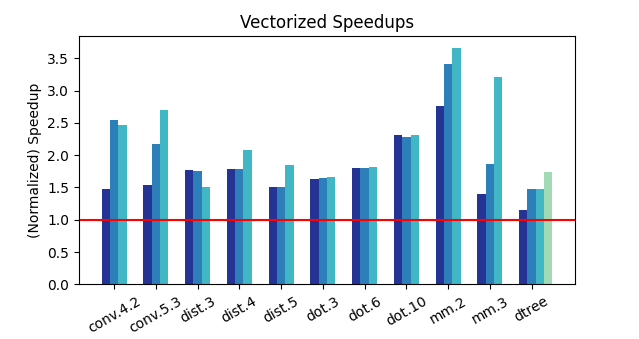
\includegraphics[width=0.9\linewidth]{figures/graphs/vector_speedups.png}
    \caption{Speedup of vectorized code over scalar (higher is better). The darkest bar for each benchmark represents unreplicated inputs, the middle bar is partially replicated, and the lightest bar is fully replicated. The light green bar for the {\tt sort[3]} and {\tt max[5]} benchmarks represent ungrouped inputs.}\label{fig:vector-speedups}
    \Description{Bar graph showing speedup from vectorization for each benchmark}
\end{figure}

% \milind{This is the punchline to your main research question: ``Can we get vectorization speedup.'' So it should be its own subsection.}
While instruction counts indicate that \system is able to effectively find vector operations for each benchmark, we must also determine whether the actual costs of rotations and blends outweigh the vectorization benefits. Hence, we run each benchmark 50 times in scalar, and 50 times after vectorization to compute the speedup from vectorization, shown in Figure~\ref{fig:vector-speedups}.
%The average speedup is computed as the total scalar execution time divided by the total vector execution time.
We find very little variance in execution time across individual runs for any benchmark.
Each benchmark has three bars representing, in order from left to right, the unreplicated, partially replicated, and fully replicated runs. 
The decision tree benchmark has an extra green bar representing the ungrouped run (without grouping, all inputs are fully replicated no matter what).
We see speedups ranging from anywhere between $1.5\times$ on the data-dense point cloud distances benchmarks to over $3.5\times$ on the highly vectorizable matrix multiply.
We also generally notice more speedup as the replication level increases, suggesting that \system is able to take advantage of replicated inputs to eliminate rotations from the schedule.

While it may appear that \system's actual speedups are sometimes well off from the idealized speedups, this is due to the rotations and blends required to implement these benchmarks outside an idealized world where vector permutation is free. For example, in the \textsf{3x3}, fully-replicated matrix multiply case, \system generates 9 rotations to move results into place. We see, though, that in benchmarks where \system can generate schedules with few rotates, it does well despite the data movement costs. For example, in \textsf{conv.4.2}, \system achieves a 2.5$\times$ speedup versus an ideal speedup of 5$\times$; and in \textsf{dot.3}, \system achieves a 1.6$\times$ speedup versus an ideal speedup of 2.7$\times$.

%\milind{This would be a good place to discuss the comparison of our speedups with rotation vs. modeled ideal speedups without rotation costs...}

\subsection{Randomly Generated Irregular Kernels}
\begin{figure}[t]
	\centering
    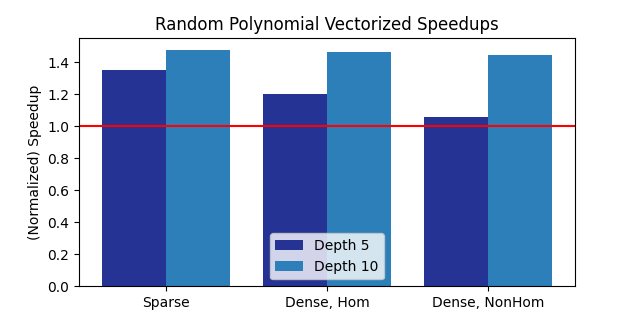
\includegraphics[width=0.9\linewidth]{figures/graphs/trees.png}
    \caption{Speedups for random polynomials (higher is better).}\label{fig:polynomial-speedups}
    \Description{Bar graph showing speedup from vectorization for randomly generated polynomials}
\end{figure}

%\raghav{How can this be said better?}
To further investigate \system's ability to vectorize, even in the absence of a regular structure on the computation, we randomly generated several polynomials to evaluate as arbitrary arithmetic expression trees.
The trees are generated according to three different regimes to cover different kinds of programs: 
\begin{enumerate}
    \item {\em Dense, homogeneous}: The expression tree is both full and complete, and all the operations are isomorphic. In principle, this represents a best case for vectorization.
    \item {\em Dense, nonhomogeneous}: The expression tree is both full and complete, each operation has a 50/50 chance of being an add or a multiply. Hence, while the trees are structurally similar, the heterogeneity of operations means that vectorization opportunities are restricted.
	\item {\em Sparse}: Many operations have one leaf node input, the tree is not very balanced. In principle, this represents a worst case for vectorization, where \system must work hard to find vectorizable computation.
\end{enumerate}
For each regime, we generate ten total polynomials, five with a circuit depth of 5 and five with a circuit depth of 10.
Each polynomial is run 20 times in scalar and 20 times after vectorization, and we average speedups across the five polynomials in each regime before reporting.
These speedups are shown in Figure~\ref{fig:polynomial-speedups}.
We see that \system is able to achieve speedups of up to $1.4\times$ by vectorizing.
Looking at the depth 5 dense nonhomogeneous polynomials, we found that many of them were too small and irregular to admit any profitable vectorization; in these cases, \system was correctly able to deduce that the scalar execution strategy was optimal rather than attempting to vectorize and incur spurious rotations.
Since the generated vector code was identical to the scalar code for several of these, the average speedup is very close to $1.0$.

We find that both sparse and dense homogeneous polynomials see substantial benefits from vectorization, with sparse polynomials having more speedup. This may seem surprising: dense homogeneous trees appear to be a best case scenario for vectorization, as all of the operations can be perfectly packed together. However, the key to this result is that rotations are expensive. The sparse trees have many vertices of arity 1---these operations do not require any rotations to align their input operands. In contrast, the dense trees require more rotations, canceling out the benefits from greater vectorization. This is further justification for \system's design decision to focus on minimizing rotation in its schedule search. In the light of this discussion, it is perhaps {\em un}surprising that the dense trees (requiring more rotation) with non-homogeneous operations (limiting vector packing) ultimately have the lowest speedup.

\subsection{Comparison to Hand-Optimized Schedules}\label{sec:expert-comparison}
To compare \system's vectorized schedules to hand-optimized baselines, we compiled three kernels with \system: matrix/vector multiply, dot product, and point-cloud distance.
Each of these kernels has a well-known expert-optimized baseline implementation, which we also implemented in \system's vector IR, before compiling both implementations to C++ and measuring the time it took to run each one 50 times.
The results are shown in Table~\ref{tab:expert-comparison-numbers}.
For smaller sizes, we see \system's vectorization was capable of matching or even outperforming the expert-written baselines, although on larger sizes the search space was often too big to automatically find the expert schedules.
Manually inspecting the generated code shows that this was usually because the schedule \system generated used one or two more rotates than the baseline.
In the case of the dot product, the schedules \system found all used the same number of rotates as the expert schedule, but occasionally incurred more blends.

\begin{table}
	\centering
    \small
    \caption{\system vectorization vs. expert-written code}\label{tab:expert-comparison-numbers}
    \begin{tabular}{lcc}
        \toprule
        Benchmark & \system time (s) & Expert time (s)\\\midrule
        mv.2 & 2.37 & 2.51 \\
        mv.3 & 3.3 & 3.9 \\
        mv.4 & 7.7 & 5.3 \\
        dist.3 & 3.5 & 3.2 \\
        dist.4 & 8.4 & 4.0 \\
        dist.5 & 15.3 & 5.5 \\
        dot.3 & 1.6 & 1.6 \\
        dot.6 & 2.9 & 2.2 \\
        dot.10 & 3.8 & 2.6 \\
        \bottomrule
    \end{tabular}
\end{table}

\subsection{Effects of Data Layout}\label{sec:effects-of-data-layout}
% \milind{Call this ``effects of data layout.'' There should be a research question in the evaluation intro that directly pertains to this case study.}
To study the effects of different data layout choices, we vary the data layout in $3\times 3$ matrix multiply:
\begin{description}
    \item[Together:] The matrices $A$ and $B$ are grouped into a single vector of $18$ elements
    \item[Separate:] $A$ and $B$ are grouped into individual vectors (this is the normal layout used in benchmarking in Figure~\ref{fig:vector-speedups})
    \item[Rows/Cols:] The rows of $A$ are grouped into three separate vectors, as are the columns of $B$.
    \item[Cols/Rows:] The columns of $A$ are grouped into three separate vectors, as are the rows of $B$.
    \item[Individual:] Each of the 18 entries are grouped into their own vector (note that this is different from simply leaving them as free scalars, because this precludes \system from choosing to put some of them on the same vector anyway).     
\end{description}
%\begin{table}
%	\centering
%    \small
%    \caption{Compilation time and vector operation counts for different layouts of $3 \times 3$ matrix muliply.} \label{tab:bigass-data-layout}
%    % \vspace{-1em}
%    \begin{tabular}{lccccc}
%    \toprule
%    Benchmark & Time (s) & VAdd+VSub & VMul & Rot & Blend\\\midrule
%    together & 584     & 5         & 2    & 15  & 10\\
%    separate & 594     & 5         & 2    & 20  & 10\\
%    rowscols & 565     & 11        & 6    & 24  & 22\\
%    colsrows & 601     & 5         & 3    & 24  & 10\\
%    indiv & 522     & 16        & 13   & 33  & 25\\\bottomrule
%    \end{tabular}
%\end{table}
In each layout, all the inputs are unreplicated.
Figure~\ref{fig:data-layout-case-study} shows the results of this case study.
Interestingly, we find that grouping the matrices together yields greater speedups than keeping them separate.
When multiple entries are on one vector, \system can arrange the elements such that rotating one automatically gives useful rotations of the others.
By contrast, when each entry is on a separate vector, every rotation must necessarily be done separately, so that schedule ends up with much more overhead. In particular, we find that {\tt indiv} requires more than twice as many rotations as {\tt together}.
%This effect can be seen in Table~\ref{tab:bigass-data-layout}: {\tt indiv} incurs over twice as many rotates as {\tt together}.
%\raghav{This is a really cool fact that I don't feel I've done justice.}\milind{This partly stems from the fact that there's something cool going on with data layout that I dont' think we fully explain in design or implementation, right? That Coyote knows that a set of inputs should go into the same vector, but actually still has the freedom to arrange them within that vector---a[0] doesn't need to be next to a[1], and so on. This should be explained in an earlier section, then reinforced here.}

\begin{figure}[t]
	\centering
    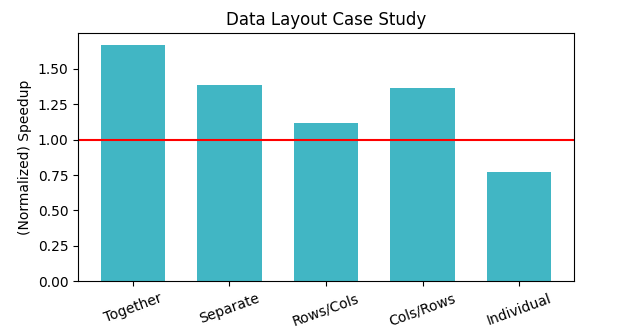
\includegraphics[width=0.9\linewidth]{figures/graphs/case_study.png}
    \caption{Speedups for the five data layout case studies (higher is better). Note that the second bar (``Separate'') corresponds to the leftmost bar of {\sf mm.3} in Figure~\ref{fig:vector-speedups}.}
    \Description{Bar graph showing speedup from vectorization for five data layout case studies}\label{fig:data-layout-case-study}
    
        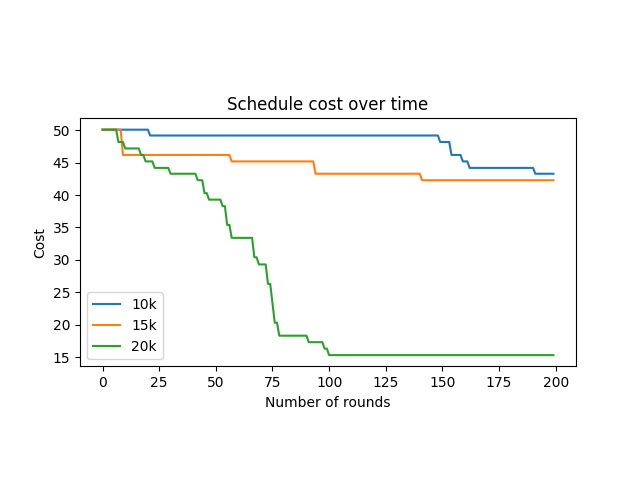
\includegraphics[width=0.9\linewidth]{figures/graphs/schedules.png}
        \vspace{-1em}
    \caption{Schedule cost over time (lower is better) for different numbers of simulated annealing iterations for data layout per step of scheduling.}
    \Description{Multiple line graphs showing the schedule cost over time for different optimization parameters}\label{fig:schedule-cost}
\end{figure}


\subsection{Effects of Search and Co-Optimization}\label{sec:search-and-cooptimization}
% % \milind{bad section title :-) Call it something like ``Effects of Search and Co-optimization.'' There should be a research question in the intro that directly pertains to the results of this study}
% % \milind{Don't just launch into the figure description. Remind people why we're here :-)}\raghav{Is this better?}
We would like to know how effective \system's schedule search strategy is, and in particular, how good of a job it does at optimizing data layout and schedule {\em together}.
To test this, we compile the 5-point distances benchmark with three different levels of data layout by varying the number of iterations of simulated annealing, and record the cost of the generated schedule during each round of the search.

Figure~\ref{fig:schedule-cost} shows the cost of the vector schedule over time for various levels of data layout.
The blue line depicts the schedule cost when we use 10k iterations of simulated annealing to find an optimal data layout at each step; the orange line is 15k iterations and the green line is 20k iterations.
As expected, doing more iterations of simulated annealing has a large effect on the efficiency of the final schedule, since we rely heavily on the fact that the data layout being used to guide each round of the search is close to optimal.
In compiling all our benchmarks, we use 20k iterations of annealing (the green line).

% The main tradeoff to be made here is one of compilation time: obviously, annealing for fewer iterations results in faster compilation, but worse schedules.
%\begin{figure}[t]
%\end{figure}


% We evaluate \system by compiling several computational kernels, of the sort that might be found in machine-learning code, and comparing their vectorized performance against an unvectorized (scalar) baseline implementation. Both the scalar and vector versions use the same FHE backend.
% Each of the matrix or vector inputs to the kernels are grouped into their own vectors as described in Section~\ref{sec:duplicating-inputs}.
%Although this can lead to worse schedules than if we didn't force groupings, we expect this to be the most common use case. \raghav{Is that what I wanna say? Or should I just combine it with the previous sentence and say ``yeah we force packings, yeah we know its not optimal.''}

% Each kernel is used in two benchmarks with differently sized inputs and three different replication strategies: once with both inputs replicated, once with only one input replicated, and once with neither input duplicated. 
% The exact benchmarks used are:
% \begin{itemize}
%     \item Matrix/Matrix multiply ($2 \times 2$ and $3 \times 3$)
%     \item Matrix/Matrix multiply followed by determinant ($2 \times 2$ and $3 \times 3$)
%     \item Pairwise distance computation (2 points and 3 points)
%     \item Vector dot product (vector size of 3 and 6)
%     \item Matrix convolution ($4 \times 4$ matrix with $2 \times 2$ kernel and $3 \times 3$ kernel)
% \end{itemize}

% % Figure~\ref{fig:ml-kernels} shows the performance results for these benchmarks.
% The red bars show the scalar execution time (normalized to 1), and the blue bars, the relative vector execution time (a smaller blue bar is better).
% Vector execution ranges from 0.77 to 6.2 times faster than scalar execution.
% Almost all benchmarks are substantially faster with vectorization, except those with lots of dependences (such as pairwise distance) or lots of reuse (such as matrix convolution), both of which result in a lot of data shuffling.

% % \milind{Start with the punchline -- don't keep people in suspense: vector execution ranges from $0.xxx$ to $y$ times faster than scalar execution. Almost all benchmarks, except those with ... have substantially faster vector than scalar runtimes, and performing full replication, which means less rotation is needed, is uniformly faster -- up to 5 times faster. Once you give them the punchline, then you can explain the rest of the details.}

% % Most of our benchmarks see a greater speedup from vectorization as we move from unreplicated inputs to fully replicated inputs.
% % This is what we expect, because, as discussed in Section~\ref{sec:duplicating-inputs}, replicating a set of inputs leads to fewer rotations necessary to get each of them to the correct lanes.
% % Performing full replication ameliorates these problems (Section~\ref{sec:duplicating-inputs}), and is uniformly faster.
% Fully-replicated vector benchmarks range from a 6.2$\times$ speedup for \texttt{mat\_mul2x2}, to an approximately $25\%$ speedup for \texttt{mat\-\_mul\-\_det3x3}

% In the unreplicated runs, we see some of the vectorized kernels (\texttt{mat\-\_convol\-\_4x4x2x2}, \texttt{mat\-\_mul\-\_det3x3}, and \texttt{pair\-wise\-\_dist2x2}) are actually {\em slower} than the scalar baseline.
% This is because the overhead of all the rotations these benchmarks incur outweighs any benefits gained from vectorization.
% In fact, it makes sense that these benchmarks would behave like that: convolution is a computation with substantial data reuse, leading to a high number of rotations to move data.
% The $2 \times 2$ pairwise distance benchmark has a fully-connected dependence graph, leading to essentially the worst case scenario for vectorization.
% And computing the determinant at the end of \texttt{mat\_mul\_det3x3} requires a reduction of 9 values, with no symmetries between them to exploit.
% However, even in these examples, the vectorized code is no more than 20\% worse than scalar, showing that despite the high rotation costs, \system is still able to properly take advantage of vectorization opportunities.
% %\raghav{This all kind of seems like a jumble but I hope I'm getting the point across}

% Overall, we see that it is almost always better to fully replicate inputs when vectorizing, unless specifically compiling several composable kernels separately. While it may seem that replicating data could increase overheads (e.g., by requiring more time to encrypt the input, or by requiring larger vector widths), in practice it does not. Encryption is vectorized in the same way as computation so does not take appreciably longer if the same data is encrypted multiple times. And vector widths in FHE are very high to begin with, so there is ample lane space to house the replicated data.

% Visually inspecting the vector code generated by \system reveals that it often automatically finds what known optimal schedules.
% For example, in the dot product kernels, \system first packs all of the multiplications into a single vector operation, then vectorizes the levels of the logarithmic reduction tree.\footnote{Note that the logarithmic reduction tree arises because the eDSL implementation of dot product uses a recursive sum operation---\system does not introduce new parallelism. Nevertheless, \system correctly exploits the parallelism that {\em does} exist in the circuit.}
% In the \texttt{mat\_mul\_det} kernels, \system first identifies the the highly vectorizable matrix multiply part of the computation, vectorizes that, and then essentially computes the highly irregular determinant on a single lane.

% \milind{Add a discussion here about visually inspecting the generated code, and point out where and whether coyote does especially cool stuff, or where it breaks down.}


% \subsection{Fuzzed Microbenchmarks}
% To investigate how various aspects of program structure affect \system's ability to vectorize, we randomly generate several expression trees according to three regimes:
% \begin{enumerate}
%     \item {\em Sparse}: Many operations have one leaf node input, the tree is not very balanced
%     \item {\em Dense, homogeneous}: The expression tree is both full and complete, and all the operations are isomorphic
%     \item {\em Dense, nonhomogeneous}: The expression tree is both full and complete, each operation has a 50/50 chance of being an add or a multiply.
% \end{enumerate}
% We generate ten trees for each regime: five with a maximum depth of 3, and five with a maximum depth of 6.
% % The relative speedups for these trees are shown in Figure~\ref{fig:fuzzed-trees}.
% We see that aside from the sparse trees of depth 3, all the rest show speedups when vectorizing, which makes sense since the sparse computations tend to be much more linear and have fewer opportunities for vectorization.
% The depth 3 trees show on average less speedup than the depth 6 trees, since they also have less work available to vectorize, and less parallelism in their circuits. %\raghav{Is this true? I'm basically trying to say that the scalar is already not bad for a tiny tree so what's the point in vectorizing it}\milind{It's basically about less parallelism. For a complete tree, parallelism is n/log(n), so as n gets bigger, there is more parallelism --- a depth 6 tree has 4 times as much parallelism as a depth 3 tree}

% \begin{figure}
%     % 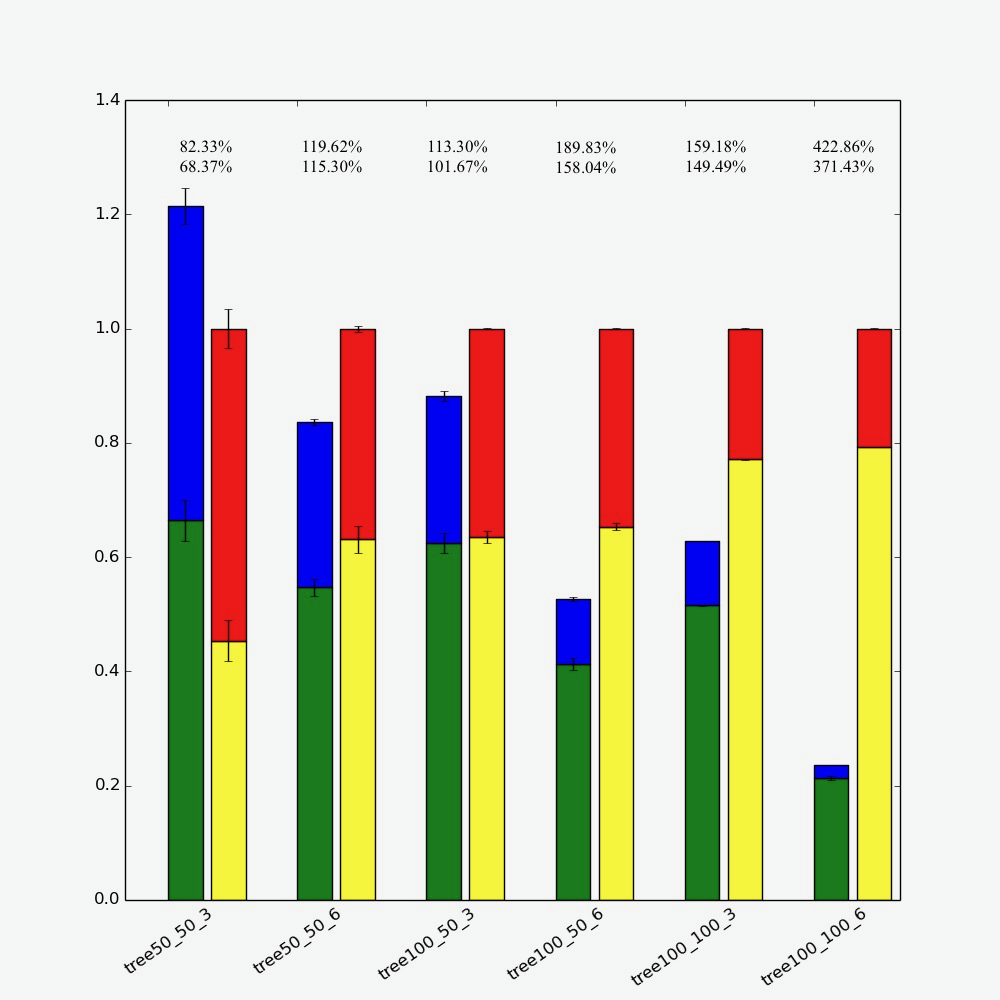
\includegraphics[width=0.9\columnwidth]{figures/graphs/TreeGraphwithNumbers.png}
%     \vspace{-0.5em}
%     \caption{Vectorization speedups on microbenchmarks. Blue/green bars represent vector time, and red/yellow bars represent (normalized) scalar time, with a smaller blue/green bar being better. Bars are split between time execution time and encryption time, with execution time on the bottom (green and yellow) and encryption time on top (blue and red). The numbers on top of the bars represent the speedup of vector over scalar, with the first one including encryption time and the second one excluding it.}\label{fig:fuzzed-trees}
% \end{figure}